\section{Meta-analysis of population prevalence with Python/PyMC}

This appendix provides code examples of how to implement the various
rate models from Chapter~\ref{TK}.  It is organized around a specific
example, the meta-analysis of the population prevalence of TK.  The
rate models are not specialized in any way for this application,
however, and the reader should keep in mind the vast generalizability
of this approach.

TK a discussion of the widespread, yet controversial belief that
schizophrenia is constant across the world and throughout time.  We
will not directly investigate that claim here, but we will lay the
foundation for such an investigation, by comparing 7 different
statistical models for a constant schizophrenia prevalence.

\subsection{The data}
To begin, the data, extracted from the results of systematic review,
<< len(d['schiz_forest.json|dexy']['r']) >> rates from <<
len(d['schiz_forest.json|dexy']['countries']) >> countries gathered
between years << d['schiz_forest.json|dexy']['min_year'] >> and <<
d['schiz_forest.json|dexy']['max_year'] >>.  Python code for dealing
with data has been unnecessarily messy in the past, and the ``Pandas''
package led by Wes McKinney is developing a DataFrame object that
changes all of this \ref{TK}.

<< d['schiz_forest.py|idio|l']['data'] >>


Figure~\ref{fig:ci-prev_meta_analysis-schiz_data} shows the data on
population prevalence of schizophrenia in males that will I have fit with
several different models, as demonstrated below.

\begin{figure}
\begin{center}
\includegraphics[width=\textwidth]{ci-prev_meta_analysis-schiz_data.png}
\end{center}
\caption{Data on population prevalence of schizophrenia in males for
  TK countries and years.  The area of the squares gives some indication the
  effective sample size of the study.}
\label{fig:ci-prev_meta_analysis-schiz_data}
\end{figure}

\subsection{Binomial model}
In PyMC, the binomial model takes the following form: <<
d['schiz_forest.py|idio|l']['binomial-model'] >>

The use of a potential instead of an observed stochastic for obs is
potentially confusing, is it \emph{actually is} an observed
stochastic, but it keeps the code quite clear, so I prefer it.

Fitting the model with PyMC's default MCMC step methods is quite
simple:
<< d['schiz_forest.py|idio|l']['binomial-fit'] >>
The following PyMC diagnostic plot shows that the model has certainly
converged when the << d['schiz_forest.json|dexy']['iter'] >>
iterations have completed:
\begin{center}
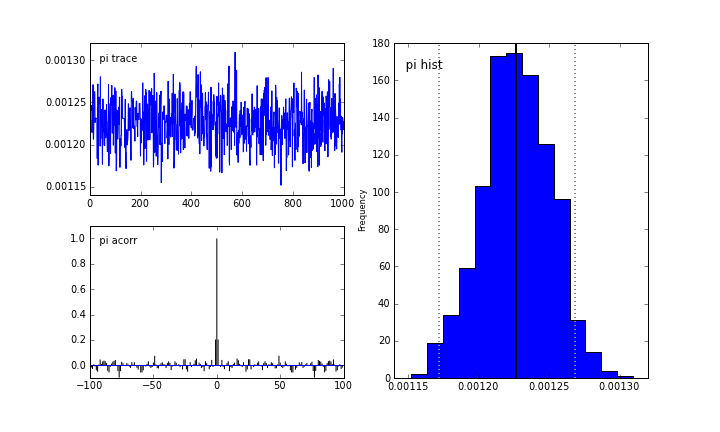
\includegraphics[width=\textwidth]{ci-prev_meta_analysis-binomial_diagnostic.png}
\end{center}


\subsection{Beta-binomial model}
Here is an implementation of the beta-binomial model in PyMC:
<< d['schiz_forest.py|idio|l']['beta-binomial-model'] >>

It is only the tiniest bit more complicated than the binomial model,
yet it is much more difficult to fit.  It requires chosing the step
method correctly (one way is shown below), and even with a
non-default step method, I ended up running it for 10 times longer
than the binomial model to ensure convergence:
<< d['schiz_forest.py|idio|l']['beta-binomial-fit'] >>

The following plot gives some evidence that it does indeed converge
with these steps and iterations:
\begin{center}
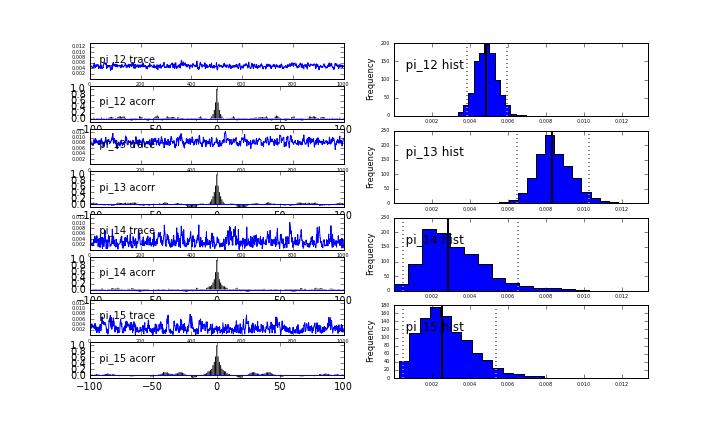
\includegraphics[width=\textwidth]{ci-prev_meta_analysis-beta_binomial_diagnostic.png}
\end{center}


\subsection{Poisson model}
The poisson model is similarly transparent in its PyMC implementation:
<< d['schiz_forest.py|idio|l']['poisson-model'] >>

Fitting it proceeds as with the binomial model.

\subsection{Negative-binomial model}
To go from the poisson model to the negative binomial one requires
only introducing an addtional stochastic node to parameterize the
over-dispersion, and switching the appropriate functions:
<< d['schiz_forest.py|idio|l']['negative-binomial-model'] >>

However, the over-dispersion stochastic diverges to extremely
over-dispersed distributions quite easily with this uninformative
prior, so I have also experimented with a number of more informative
priors, designed to represent the expert belief that there is some
value to the data, even if it has ten-fold variation for measurements
of what is believed to be the same rate.  Here is the approach which I
have settled on for now:
<< d['poisson_model.py|idio|l']['negative-binomial_dispersion-alt_prior'] >>

\subsection{Normal model}
I'm not a huge fan of the normal model, and it seems like this
approach is questionable.  In particular, there are many alternative
ways to include the sampling variation, and I'm not sure that there is
any reason to prefer one.  I've chosen a simple approach that
decomposes the total variation in the observed data into part that
comes from the statistical sampling and part that comes from
everything else (which I could call ``non-sampling variation'').  The
model is simple, but maybe something else would be simple and better:
<< d['schiz_forest.py|idio|l']['normal-model'] >>



\subsection{Log-normal model}
By taking logs of the data and the parameter, the normal model can be
converted to a log-normal model, which at least does not have positive
likelihood for negative rate data.  This approach will not work with
rate values of zero, however:
<< d['schiz_forest.py|idio|l']['log-normal-model'] >>

It is possible to substitute in any other monotonic transform instead
of $\log$ here, to produce another similar model.  Logit and Probit
models, for example.



\subsection{Offset log-normal model}
One way to deal with the shortcoming of the log-normal model, its
inability to accept rate values of zero, is the offset log-normal,
which is implemented in PyMC as follows:
<< d['schiz_forest.py|idio|l']['offset-log-normal-model'] >>

This model is quite flexible, but I haven't seen it used in the
literature, so I'm not sure how it will be received.

